\documentclass{article}
\usepackage[landscape]{geometry}
\usepackage{url}
\usepackage{multicol}
\usepackage{amsmath}
\usepackage{esint}
\usepackage{amsthm}
\usepackage{amsfonts}
\usepackage{tikz}
\usetikzlibrary{decorations.pathmorphing}
\usetikzlibrary{graphs}
\usetikzlibrary{shapes}
\usetikzlibrary{backgrounds}
\usetikzlibrary{calc}
\usetikzlibrary{patterns}
\usetikzlibrary{positioning, fit, arrows.meta}
\usepackage{amsmath,amssymb}
\usepackage{subcaption}
\usepackage[english]{babel}
\usepackage{enumitem}


\usepackage{colortbl}
\usepackage{xcolor}
\usepackage{mathtools}
\usepackage{amsmath,amssymb}
\usepackage{enumitem}
\makeatletter

\newcommand*\bigcdot{\mathpalette\bigcdot@{.5}}
\newcommand*\bigcdot@[2]{\mathbin{\vcenter{\hbox{\scalebox{#2}{$\m@th#1\bullet$}}}}}
\makeatother

\title{Discrete Exam 2 Note Sheets}
\usepackage[utf8]{inputenc}

\advance\topmargin-.8in
\advance\textheight
3in
\advance\textwidth3in
\advance\oddsidemargin-1.40in
\advance\evensidemargin-1.45in
\parindent0pt
\parskip1pt
\newcommand{\hr}{\centerline{\rule{3.5in}{1pt}}}

% Natural Numbers 
\newcommand{\N}{\ensuremath{\mathbb{N}}}

% Whole Numbers
\newcommand{\W}{\ensuremath{\mathbb{W}}}

% Integers
\newcommand{\Z}{\ensuremath{\mathbb{Z}}}

% Rational Numbers
\newcommand{\Q}{\ensuremath{\mathbb{Q}}}

% Real Numbers
\newcommand{\R}{\ensuremath{\mathbb{R}}}

% Complex Numbers
\newcommand{\C}{\ensuremath{\mathbb{C}}}

\begin{document}





















\begin{center}{\huge{\textbf{Discrete Final Exam Note Sheets}}}\\
\end{center}
\begin{multicols*}{2}

\tikzstyle{mybox} = [draw=black, fill=white, very thick,
    rectangle, rounded corners, inner sep=5pt, inner ysep=10pt]
\tikzstyle{innerbox} = [draw=black, fill=gray!20, thick,
    rectangle, rounded corners, inner sep=5pt, inner ysep=10pt]
\tikzstyle{fancytitle} =[fill=black, text=white, font=\bfseries]

%------------ Measures of Center ---------------
\begin{tikzpicture}
\node [mybox] (box){%
    \begin{minipage}{0.46\textwidth}

        \underline{\textbf{Definitions}}: \\
        
    	\begin{tabular}{lp{10.2cm} l}
        	\textit{Vertices}:
            & Points defined on a graph. \\
            \textit{Degree}: 
            & Number of edges that include the vertex. \\
            \textit{Loop}: 
            & An edge which connects a vertex to itself. \\
            \textit{Adjacent}: 
            & If two vertices are adjacent, then there is a single edge between them. \\
            \textit{Path}:
            & A sequence of adjacent vertices. \\
            \textit{Circuit}:
            & A path with the same initial starting and ending vertex. \\
            \textit{Connected}:
            & If each vertex can be reached by path from each other, then they are connected.
    	\end{tabular}
    
        \textbf{Notes}: 
        If all degrees are even, you can start anywhere, and you will end there (circuit). If you have exactly 2 points of odd degree, you can do it by starting at one end, and ending at the other. For the missing case of vertices (exactly 1 point of odd degree), there cannot be a single vertex of odd degree.
    
        \vspace{0.3cm}
    
        \begin{tabular}{lp{10cm} l}
        	\textbf{\textit{Theorem 1}}: &
            The sum of the degrees is always twice the number of edges.\\
            \textit{Corollaries}: &
            The sum of degrees are always even. (AND) No graph has a single vertex of odd degree.       
    	\end{tabular}
    
        \begin{minipage}{\textwidth}
            \begin{tikzpicture}[>=stealth, scale=0.5] % Arrow tip style for the first picture
                \node[anchor=south] at (1,1.6) {\underline{\textbf{Directed Graph (Diagram)}}:};
            
                        \node[draw, circle, fill=white, inner sep=3.5pt] (A) at (0,0) {A};
                        \node[draw, circle, fill=white, inner sep=3.5pt] (B) at (4,0) {B};
                        \node[draw, circle, fill=white, inner sep=3.5pt] (C) at (4,-4) {C};
                        \node[draw, circle, fill=white, inner sep=3.5pt] (D) at (0,-4) {D};
                        
                        % Draw rectangle edges with arrows
                        % \draw[parameters] (fromWhere) -- (toWhere);
                        \draw[thick,->] (A) -- (B);
                        \draw[thick,->] (B) -- (C);
                        \draw[thick,->] (C) -- (D);
                        \draw[thick,->] (D) -- (A);
                        
                        % Draw diagonal from A to C with arrow
                        \draw[thick, ->] (A) -- (C);
                
                        % Add loop from left to right on vertex A
                        \draw[thick, ->] (A) to [out=180,in=90,looseness=8] (A);
                
            \end{tikzpicture}
        \hfill % Space between the two tikzpictures
        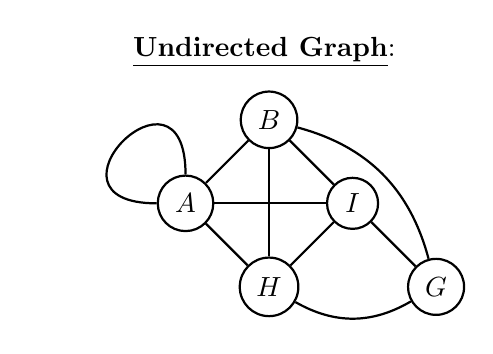
\begin{tikzpicture}[node distance={15mm}, thick, main/.style = {draw, circle, inner sep=3.5pt, execute at begin node=$, execute at end node=$}]
            \node[anchor=south] at (1,1.6) {\underline{\textbf{Undirected Graph}}:};
                % Nodes
                \node[main] (A) {A};
                \node[main] (B) [above right of=A] {B};
                \node[main] (I) [below right of=B] {I};
                \node[main] (H) [below left of=I] {H};
                \node[main] (G) [below right of=I] {G};
                
                % Lines
                % \draw[parameters] (fromWhere) -- (toWhere);
                \draw (A) -- (B);
                \draw (A) -- (I);
                \draw (A) -- (H);
                \draw (B) -- (I);
                \draw (B) -- (H);
                \draw (G) -- (I);
                \draw (H) -- (I);
                
                \draw (B) to [bend left] (G);
                \draw (H) to [bend right] (G);
                
                \draw[thick] (A) to [out=180,in=90,looseness=8] (A);
            \end{tikzpicture}
        \end{minipage}


	
    \end{minipage}
};
%------------ Measures of Center Header ---------------------
\node[fancytitle, right=10pt] at (box.north west) {2.1 Graphs};
\end{tikzpicture}


%------------ Measures of Variability ---------------
\begin{tikzpicture}
\node [mybox] (box){%
    \begin{minipage}{0.46\textwidth}

    \underline{\textbf{Definitions}}: \\
    
	\begin{tabular}{lp{8cm} l}
    	\textit{Set}:
        & Collection of objects, called \textit{elements}, or \textit{members}. \\
        \textit{Predicate}: 
        & A set whose elements are exactly the elements of \textit{A} for which $s(x)$ is true.
        For example, $\{x\in A\colon P(x)\}$ where $P$ is any predicate with $A$ as its domain. \\
        \textit{Equals}:
        & If \textit{A} is \textit{equal} to \textit{B}, then $x\in A \iff x\in B$. \\
        \textit{Subset}:
        & If $A$ is a subset of $B$, then if $x\in A$, then $x\in B$. \\
        \textit{Empty set}:
        & The set with no elements: if $x$ exists, then $x\notin \emptyset$.
	\end{tabular} \\

    \textbf{Note}: An example of a predicate could be $A = \{1,3,5,7,9\}$, then $\{x\in A\colon x^2 < 10\} = \{1,3\}$. This is called set builder notation. 

    \end{minipage}
    };
%------------ Measures of Variability Header ---------------------
\node[fancytitle, right=10pt] at (box.north west) {2.2 Sets};
\end{tikzpicture}


%------------ Discrete Random Variable and Distributions ---------------
\begin{tikzpicture}
\node [mybox] (box){%
    \begin{minipage}{0.46\textwidth}
    
    \underline{\textbf{Theorems}}: \\

    \begin{tabular}{lp{10cm} l}
    	\textbf{\textit{Theorem 2}}:
        & Suppose $A,B$ and $C$ are sets with $A = B$ and $B = C$. Then $A = C$ \\
	\end{tabular}
    \begin{proof}
        Let $x\in A$. Since $A = B, x\in B$. Since $B=C$, then $x\in C$. Now, let $y\in C$. Since $B=C, y\in B$. Since $A=B$ then $y\in A$. $\therefore A=C$
    \end{proof}
    \begin{tabular}{lp{8cm} l}
        \textbf{\textit{Theorem 3}}:
        & \textit{A} is a set, \textit{P} is a predicate. $\{x \in A \colon P(x) \} \subseteq A$ \\
        \textbf{\textit{Theorem 4}}: 
        & Let $A$ and $B$ be sets. Then, $A\subseteq B \iff A\cap B = A$.
	\end{tabular} \\
    \begin{proof}
        ($\Rightarrow$)
        Show that if $A\subseteq A\cap B = A$ Let $x\in A\cap B$. Then, $x\in A$ and $x\in B$. $\therefore$ $x\in A$. Let $y\in A$. Since, $A\subseteq B$, $y\in B$. So, $y\in A$ and $y\in B$. $\therefore y\in A\cap B$. \\
        \noindent \textit{Proof.} ($\Leftarrow$) \\
        Show that $A\cap B = A$ then, $A\subseteq B$. Let $x\in A$. Since $A = A\cap B$, $x\in A\cap B$. So, $x\in A$ and $x\in B$. $\therefore x\in B$.
    \end{proof}
    
    \underline{\textbf{Definitions (cont.)}}: \\

    \begin{tabular}{lp{9.8cm} l}
        \textit{Union}:
        & $A\cup B\colon x\in A\cup B$ if $x\in A$ or $x\in B$ \\
        \textit{Intersection}: 
        & $A\cap B\colon x\in A\cap B$ if $x\in A$ and $x\in B$. \\
        \textit{Product}: 
        & $A\times B$ is the set of all ordered pairs, $(a,b)$, where $a\in A, b\in B$, such that if $A = \{1,2\}, B = \{2,4,6\}$, then $A\times B = \{(1,2),(1,4),(1,6),(2,2),(2,4),(2,6)\}$ \\
        \textit{Complement}: 
        & Suppose $A \subseteq U$. $A'$ relative to $U$ is $\{x\in U \colon x \notin A\} = A'$.
    \end{tabular} \\
	
	
    \end{minipage}
};
%------------ Discrete Random Variable and Distributions Header ---------------------
\node[fancytitle, right=10pt] at (box.north west) {2.2 Sets (cont.)};
\end{tikzpicture}


%------------ Sets and Probability ---------------
\begin{tikzpicture}
\node [mybox] (box){%
    \begin{minipage}{0.46\textwidth}

        \underline{\textbf{Definitions}}: \\
        
        \begin{tabular}{lp{10cm} l}
            \textit{Functions}:
            & A \textit{function} is the association $x\in X$, with a unique $y\in Y$. Denoted as $f(x) = y$. \\
            \textit{One-to-one}:
            & $f$ is \textit{one-to-one} if for each $x_1, x_2 \in X$, if $f(x_1) = f(x_2)$, and $x_1 = x_2$.  \\
            \textit{Onto}: 
            & $f$ is onto if there exists an $x\in E$ so that $f(x) = y$. \\
        \end{tabular} \\
    
        \begin{minipage}{\textwidth}
            \begin{tikzpicture}[>=stealth, scale=0.7] % Arrow tip style for the first picture
                \node[anchor=south] at (1,1) {\underline{\textbf{One-to-One Graph}}:};
                    \node[draw, circle, fill=white, inner sep=2pt] (A) at (0,0) {};
                    \node[draw, circle, fill=white, inner sep=2pt] (B) at (0,-1) {};
                    \node[draw, circle, fill=white, inner sep=2pt] (C) at (0,-2) {};
                    \node[draw, circle, fill=white, inner sep=2pt] (D) at (2,0) {};
                    \node[draw, circle, fill=white, inner sep=2pt] (E) at (2,-1) {};
                    \node[draw, circle, fill=white, inner sep=2pt] (F) at (2,-2) {};

                    \draw[thick,->] (A) -- (D);
                    \draw[thick,->] (B) -- (E);
                    \draw[thick,->] (C) -- (F);
                
                    % Surround Nodes A and B with a box labeled F
                    \node[draw, rectangle, fit=(A) (C), inner sep=12pt, label=left:F] (BoxF) {};
                    
                    % Surround Nodes C and D with a box labeled Y
                    \node[draw, rectangle, fit=(D) (F), inner sep=12pt, label=right:Y] (BoxY) {};
                
            \end{tikzpicture}
        \hfill % Space between the two tikzpictures
            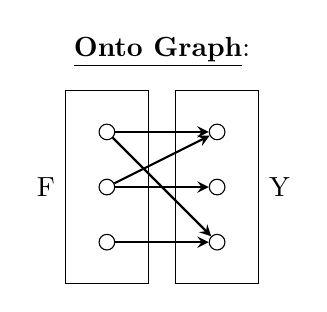
\begin{tikzpicture}[>=stealth, scale=0.7]
                \node[anchor=south] at (1,1) {\underline{\textbf{Onto Graph}}:};
            
                \node[draw, circle, fill=white, inner sep=2pt] (A) at (0,0) {};
                \node[draw, circle, fill=white, inner sep=2pt] (B) at (0,-1) {};
                \node[draw, circle, fill=white, inner sep=2pt] (C) at (0,-2) {};
                \node[draw, circle, fill=white, inner sep=2pt] (D) at (2,0) {};
                \node[draw, circle, fill=white, inner sep=2pt] (E) at (2,-1) {};
                \node[draw, circle, fill=white, inner sep=2pt] (F) at (2,-2) {};

                
                % Draw rectangle edges with arrows
                \draw[thick,->] (A) -- (D);
                \draw[thick,->] (A) -- (F);
                \draw[thick,->] (B) -- (D);
                \draw[thick,->] (B) -- (E);
                \draw[thick,->] (C) -- (F);
            
                % Surround Nodes A and B with a box labeled F
                \node[draw, rectangle, fit=(A) (C), inner sep=12pt, label=left:F] (BoxF) {};
                
                % Surround Nodes C and D with a box labeled Y
                \node[draw, rectangle, fit=(D) (F), inner sep=12pt, label=right:Y] (BoxY) {};
                    
            \end{tikzpicture}
        \end{minipage}
    
	
    \end{minipage}
};
%------------ Sets and Probability Header ---------------------
\node[fancytitle, right=10pt] at (box.north west) {2.3 Functions};
\end{tikzpicture}


%------------ Continuous Random Variable and Distributions ---------------
\begin{tikzpicture}
\node [mybox] (box){%
    \begin{minipage}{0.46\textwidth}

    \underline{\textbf{Onto and One-to-One Examples}}:
    
	\begin{enumerate}
	\setlength\itemsep{0em}
        \item Let $f\colon \mathbb{N} \rightarrow \mathbb{N}$ by $f(x) = 3n + 1$. Then $f$ is one-to-one. \\
        
        Let $x_1,x_2\in \mathbb{N}$ so that $f(x_1) = f(x_2)$. We hope to show $x_1 = x_2$. $f(x_1) = 3x_1 + 1$ and $f(x_2) = 3x_2 + 1$. Then, 
        \begin{align*}
            3x_1 + 1 &= 3x_2 + 1 \\
            3x_1 &= 3x_2 \\
            x_1 &= x_2
        \end{align*}
        Therefore, $f$ is one-to-one.
        \item Suppose that each of $f\colon B \rightarrow C$ and $A \rightarrow B$ are one-to-one and onto functions. Let $h \colon A \rightarrow C$ be defined as $h = f \circ g$.
        \begin{enumerate}
            \item Show that $h$ is one-to-one.

            Let $x_1, x_2 \in A$ and suppose $h(x_1) = h(x_2)$. By definition of \textit{h}, $h(x_1) = f(g(x_1))$ and $h(x_2) = f(g(x_2))$. $\therefore f(g(x_1)) = f(g(x_2))$. Now, since $f$ is one-to-one, $f(g(x_1)) = f(g(x_2)) \rightarrow g(x_1) = g(x_2)$. And since $g$ is one-to-one as well, $g(x_1) = g(x_2)$ and $x_1 = x_2$. \\

            \item Show that $h$ is onto.

            Let $c\in C$. Since \textit{f} is onto, there exists $b\in B \colon f(b) = c$. And by the same logic, since $g$ is onto, for this $b\in B$, $\exists a\in A \colon g(a) = b$. Now, consider $h(a) = f(g(a)) = f(b) = c$, by substitution. Thus, $\forall c \in C, \exists a \in A \colon h(a) = c$. $\therefore$ \textit{h} is onto.
        \end{enumerate}
        \item Find functions for all $f,g,h \colon \mathbb{Z} \rightarrow \mathbb{Z}$ so that (a) \textit{f} is one-to-one and not onto, (b) \textit{g} is not one-to-one and is onto, and\dots
        \begin{enumerate}
            \item Let f(x) = 2x. Assume $f(x_1) = f(x_2)$. Then $2x_1 = 2x_2$. Then, $x_1 = x_2$. Therefore, \textit{f} is one-to-one. Now, let $y,k \in \mathbb{Z} \colon y = 2k + 1$ (\textit{y} is odd). There is no integer \textit{x} such that $2x=2k +1$ because the left side is always even, and the right side is always odd. $\therefore f$ is not onto.
            \item Consider the piece-wise function, 
            \[
            g(x) = 
            \begin{cases} 
            \frac{x}{2} & \text{if } x \text{ is even}, \\
            \frac{-(x+1)}{2} & \text{if } x \text{ is odd}.
            \end{cases}
            \]
            If $y\geq 0$, let $y = 2y$. Then $g(x) = g(2y) = y$ because \textit{x} is even by definition. If $y < 0$, let $x = -2y - 1$. Then $g(x) = g(-2y-1) = \frac{-(2y-1)}{2} = y$ because $x$ is odd by definition $\therefore$ for any $y\in \mathbb{Z}, \exists x\colon g(x) = y, \therefore g$ is onto. Now, consider $x_1 = 2$ and $x_2 = -3$. Then $g(2) = \frac{2}{2} = 1$ and $g(-3) = \frac{-((-3) + 1}{2} = 1$. Since $2 \ne 3$, $x_1 \ne x_2 \therefore g$ is not one-to-one.
        \end{enumerate}
    \end{enumerate}
	
    \end{minipage}
};
%------------ Continuous Random Variable and Distributions Header ---------------------
\node[fancytitle, right=10pt] at (box.north west) {2.3 Functions (cont.)};
\end{tikzpicture}


%------------ Summarizing Main Features of f(x) ---------------
\begin{tikzpicture}
\node [mybox] (box){%
    \begin{minipage}{0.46\textwidth}

    \begin{enumerate}
    \setcounter{enumi}{2}
    \item \dots \textit{h} is neither.
        \begin{enumerate}
            \setcounter{enumii}{2}
            \item Consider $h(x) = x^2$. Let $x_1 = -1$, and $x_2 = 1$. $h(-1) = 1$ and $h(1) = 1$. Hence, $x_1 \ne x_2$ and is not one-to-one. Because $h(x)$ only produces positive numbers, it cannot cover every possible integer, and hence, $h(x) \ne y$ for $y \in \mathbb{Z} \therefore h$ is not onto.
        \end{enumerate}
    \end{enumerate}
    
	
    \end{minipage}
};
%------------ Summarizing Main Features of f(x) ---------------------
\node[fancytitle, right=10pt] at (box.north west) {2.3 Functions (cont.)};
\end{tikzpicture}


%------------ Sum and Average of Independent Random Variables ---------------
\begin{tikzpicture}
\node [mybox] (box){%
    \begin{minipage}{0.46\textwidth}
     \underline{\textbf{Definitions}}: \\
        
        \begin{tabular}{lp{8.7cm} l}
            \textit{Relation}:
            & Defined as $r \colon X \rightarrow Y$ if $R \subseteq X \times Y$. \\
            \textit{Reflexive}:
            & If for each $x\in X$, $x \ R \ x$. \\
            \textit{Symmetric}:
            & If when $a \ R \ b$, then $a\ R \ b$. \\
            \textit{Transitive}: 
            & If when $a \ R \ b$, and $b \ R \ c$, then $a \ R \ c$. \\
            \textit{Equivalence relation}:
            & Has all three above traits. \\
            \textit{Equivalence class}:
            & Because equivalence relations allow us to partition the domain, each partition is then labeled as $[a]$. \\
            \textit{Modulo (\%)}:
            & For two integers, \textit{a} and \textit{b}, \textit{a} is said to be equivalent to \textit{b} modulo \textit{n} if the difference between \textit{a} and \textit{b} (that is, $a-b$) is divisible by \textit{n}. This means there exists an integer \textit{k} such that $a-b = kn$.
        \end{tabular} \\
        
        \textbf{Note}: All functions are relations, but not all relations are functions. Abiding by the definition of a function, if $x$ can be mapped to more than one $y$-value, the statement is not a function. Also note for the relation traits, those items are true on the basis that $R\colon X \rightarrow X$ is a relation.

        \begin{center}\textbf{Prove Modulo Is an Equivalence Class}
        \end{center}
        Let $n\in \mathbb{N}$, and let $a,b,c\in \mathbb{Z}$. 
        \begin{itemize}
            \item Is $a\equiv a \mod{n}$ reflexive? $a-a = 0$, which is divisible by \textit{n}. So, Yes.
            \item Is $a\equiv a \mod{n}$ symmetric? Well, we must find out if $a\equiv b \mod {n}$ is equivalent to $b\equiv a \mod{n}$. We know that $(a-b)$ is divisible by \textit{n}, and there are no restrictions to also include that $b- a$ is also divisible by $n$. Yes.
            \item Is $a\equiv a \mod{n}$ transitive? Let $a \equiv b \mod{n}$ and $b \equiv c \mod{n}$. This means that $a = b + kn$ and $b = c + ln$ for some integers \textit{k} and \textit{l}. Substituting the second equation into the first, we find that $a = (c + ln) + kn = c + (l + k)n$. So, $a\equiv c \mod{n}$, as required for transitivity.
        \end{itemize}
        \begin{center}\textbf{Integers Modulo \textit{n}}
        \end{center}
        The set of equivalence classes form by this equivalence relation is called the \textit{integers modulo n}, and is denoted as $\mathbb{Z} /n$. We use $[k]$ to denote the equivalence class of $[k]$. For example, elements of $\mathbb{Z} \ 3$ are $[0] = \{\dots, -9, -8, -6, -3, 0, 3, 6, 9,\dots \}, \text{ and } [1] = \{\dots, -8,-5,-2,1,4,7,10, \dots \}$.
    \end{minipage}
};
%------------ Sum and Average of Independent Random Variables ---------------------
\node[fancytitle, right=10pt] at (box.north west) {2.4 Relations};
\end{tikzpicture}


%------------ Maximum and Minimum of Independent Variables ---------------
\begin{tikzpicture}
\node [mybox] (box){%
    \begin{minipage}{0.46\textwidth}
    
    \underline{\textbf{Definitions}}:
    \begin{center} \textbf{Graphs} \\
    \end{center}
    \begin{tabular}{lp{10cm} l}
            \textit{Graph}:
            & $G = (V,E)$, is a pair of sets $V$, the \textit{vertex set}, and \textit{E} the \textit{edge set}, so that each element of \textit{E} has the form $\{v_i,v_j\}, v_1, v_j \in V$. \\
            \textit{Degree}:
            & The number of edges which include $v$. Granted that $v\in V$. \\
            \textit{Adjacent}:
            & Vertices $u, v$ belong to $\{u,v\} \in E$. \\
            \textit{Path}:
            & From vertex $v_0$ to vertex $v_n$ is a sequence $v_0, v_1, v_2 \dots, v_n$, where each $v_i \in V$ and $\{v_i,v_{i+1}\} \in E$. \\
            \textit{Simple}:
            & No edge occurs twice in a path. \\
            \textit{Connected}: 
            & If each pair of vertices are adjoined by an edge. \\
        \end{tabular} 

    \begin{center} \textbf{Circuits} \\
    \end{center}

    \begin{tabular}{lp{10cm} l}
        \textit{Circuit}: 
        & A path with the same starting and ending vertex. \\
        \textit{Complete}:
        & On $n$ vertices, $K_n$, is the connected graph where each vertex is adjacent to each other. \\
    \end{tabular}

    \begin{center}\textbf{Bipartite Graphs} \\
    \end{center}
    
    \begin{tabular}{lp{10cm} l}
    
        \textit{Bipartite}:
        & The vertex set $V = v_1 \cup v_2, v_1 \cap v_2 = \emptyset$, and no vertex in $V_1$ is adjacent to any other in $V_1$, and no vertex in $V_2$ is adjacent to any other in $V_2$.
    \end{tabular}

    \begin{center}\textbf{Trees} \\
    \end{center}
    
    \begin{tabular}{lp{10cm} l}
        \textit{Tree}:
        & A connected graph that has no circuit. \\
        \textit{BiSTree}:
        & For every node, all elements in the left subtree are less than the node's value, and all elements in the right subtree are greater. \\
        \textbf{\textit{Lemma}}: 
        & If $G$ is a tree, $G$ has at least one vertex of degree 1.
    \end{tabular}
    \begin{proof}
         For the sake of contradiction, suppose each vertex has degree $\geq 2$. Pick a vertex, $v_0$. Since, $\deg(v_0) \geq 2$, it is adjacent to some $v_j$. Because $\deg(v_1) \geq 2$, it has an edge distinct from $\{v_0,v_1\}$, follow it to $v_2$. Then, $v_2$ has edge distinct from $\{v_1,v_2\}$, follow it to $v-3$. If $v_3=v_0 (v_1,v_2)$ we have a circuit. $v_3$ has edge distinct from $\{v_2,v_3\}$. Go to $v_4$. Continue \dots. Either some $v_j$ is visited again, or $v_0,v_1,v_2,\dots v_n$. Therefore, it must be a circuit. \\

        Hence, $G$ must have a vertex with degree of at least 1 such that $1\leq$.
    \end{proof}
    \begin{tabular}{lp{10cm} l}
        \textbf{\textit{Theorem 1}}:
        & A tree with \textit{n} vertices always has $n - 1$ edges.
    \end{tabular} 
    \begin{proof}
        By the Lemma, there exists a vertex of degree 1. Remove it and its edge. We still have a tree. This new tree has vertex of degree 1. Remove it and its edge. Continue until you get to $k_2$, then $k_1$. We stop with 1 vertex, 0 edges, we have removed $n-1$ vertices. Each edge was removed. Thus, we threw out \textit{all} $n-1$ edges.
    \end{proof}
    
    \end{minipage}
};
%------------ Maximum and Minimum of Independent Variables ---------------------
\node[fancytitle, right=10pt] at (box.north west) {2.6 Graph Theory};
\end{tikzpicture}


%------------ Some Continuous Distributions ---------------
\begin{tikzpicture}
\node [mybox] (box){%
    \begin{minipage}{0.46\textwidth}

    \begin{center}\textbf{Euler Circuits} \\
    \end{center}
    
    \begin{tabular}{lp{9cm} l}
        \textit{Euler circuit}:
        & A circuit graph which uses each edge only once. \\
        \textit{Euler path}:
        & A path which uses each edge -- start and end vertices are distinct.
    \end{tabular} \\
    
    \textbf{Note}: $G$ has an Euler circuit if, and only if, it is connected and each vertex has an even degree. Intuitively, if each vertex has an even degree, then if you come into the vertex through the entrance (first edge), and you leave through the exit (second edge) you have used up both openings. \\
    
    $G$ has an Euler path if, and only if, it is connected and has exactly two vertices of odd degree.

    \begin{center}\textbf{Isomorphisms} \\
    \end{center}
    Two graphs, $G = (V,E)$ and $H = (W,f)$ are \textit{isomorphic} if there is an $f\colon V\rightarrow W$ which is one-to-one, onto, and $\{v_i, v_j\} \in E \iff \{f(v_i), f(v_j)\} \in F$.

    \begin{center}\textbf{Vertex Colorings} \\
    \end{center}
    If $G$ contains a triangle (i.e., if it has a copy of $k_3$), we need at least 3 colors. If $G$ contains a copy of $K_n$, we need at least $n$. \\

    If a graph has no overlapping paths, the graph requires no more than 4 colors.

    \begin{center}\textbf{Hamilton Graphs} \\
    \end{center}
    A graph has a \textit{Hamilton Circuit} if there is a circuit that uses each vertex once. \\

    \textbf{Note}: This is different from Euler, as Euler uses edges. This is specifically for vertices. If it has a vertex of degree 1, it cannot have a Hamilton circuit.

    

    
    
    \end{minipage}
};
%------------ Some Continuous Distributions Header ---------------------
\node[fancytitle, right=10pt] at (box.north west) {2.6 Graph Theory (cont.)};
\end{tikzpicture}


%------------ Normal Distribution ---------------
\begin{tikzpicture}
\node [mybox] (box){%
    \begin{minipage}{0.46\textwidth}

    \begin{center}\textbf{Sets}
    \end{center}

    \begin{enumerate}
        \item Suppose that the universal set $U = \{1,2,3,4,5,6,7,8,9,10\}$ and the particular sets $A = \{2,3,5\}$ and $B = \{1,3,5,7,9\}$. Find each of the following:
        \begin{enumerate}
            \item $A \cup B = \{1,2,3,5,7,9\}$
            \item $A \cap B = \{3,5\}$
            \item $\{x\in U \colon x^2 < 10 \land x \in A\} = \{2,3\}$
            \item $B' \cap A = \{2\}$
            \item $\{x \in A \colon x \geq 7\} = \emptyset$
            \item $\mathcal{P}(A) = \{\emptyset, \{2\}, \{3\}, \{5\}, \{2,3\}, \{2,5\}, \{3,5\}, \{2,3,5\}\}$
        \end{enumerate}
    \end{enumerate}
    
    \end{minipage}
};
%------------ Normal Distribution Header ---------------------
\node[fancytitle, right=10pt] at (box.north west) {Extra Examples \& Proofs};
\end{tikzpicture}


%------------ Bernoulli and Binomial Random Variables ---------------
\begin{tikzpicture}
\node [mybox] (box){%
    \begin{minipage}{0.46\textwidth}

    \begin{enumerate}
    \setcounter{enumi}{1}
        \item Show that for any two sets \textit{A} and \textit{B}, $A\cap B\subseteq A$. \\
        
        Suppose $A$ and $B$ are sets. Let $x\in A\cap B$. By the definition of intersection, this means $x\in A$ \underline{and} $x\in B$. Since $x\in A$, it follows that every element in $A\cap B$ is also in \textit{A}. Thus, by the definition of subset, $A\cap B \subseteq A$.
        \item Let \textit{A} and \textit{B} be sets. Show that $A\subseteq B \iff A\cup B = B$. \\
        $(\Rightarrow)$ \\
        
        Suppose $A$ and $B$ are sets such that $A\subseteq B$. Then, if $x\in A$, then $x\in B$ by the given information. Then, if $x\in B$, then $x\in A\cup B$, and if $x\in A\cup B$, then $x\in A \cup B$, by definition of union. Since, $x\in A$ implies $x\in B$, by definition of subset, and since $x\in A\cup B$ implies $x\in B$, then $A\cup B = B$. \\
        $(\Leftarrow)$ \\
        
        Suppose \textit{A} and \textit{B} are sets such that $A \cup B = B$. Let $x\in A$ by assumption. Then, by the definition of union, $x\in A$ implies $x\in B$. And since $A \cup B = B$, $x\in A\cup B$ implies $x\in B$, and similarly, $x\in A$ implies $x\in B$. Therefore, by definition of subset, $A \subseteq B$.
    \end{enumerate}

    \begin{center} \textbf{Relations and Functions}
    \end{center}

    \begin{enumerate}
        \item Determine if $\mathbb{R} \rightarrow \mathbb{R}$ by $x \ R \ y \iff x^2 = y$ is a function or relation. \\
        
        This is a \textbf{function} because each input \textit{x}, has only one output. For example, consider $x = -1, 1$, then $y = 1$.
        \item  Determine if $\mathbb{R} \rightarrow \mathbb{R}$ by $x \ R \ y \iff x^2 = y$ is a function or relation. \\
        
        This is a \textbf{relation} because one $x$-value maps to several $y$-values. Consider $x = 1$, then $y = 1, -1$.
        \item Suppose $R\colon A\rightarrow A$ is symmetric and transitive. $\text{Must } R \text{ be reflexive?}$ \\
        
        No, it does not have to be reflexive. \\

        Consider $A = \{1,2,3\}$ and a relation $R$ defined as $\{(1,2),(2,1),(1,1),(2,2)\}$. This relation is symmetric because if $(1,2)\in R$, then $(2,1)\in R$, and if $(1,1)\in R$ then $(2,2)\in R$, and vice versa. It is also transitive because since $(1,1), (2,2)$ is in $R$, so is $(1,2),(2,1)$. That being said, since $a\in A$, and for it to be reflexive, $3\in R$, which is not present.
    \end{enumerate}

    \end{minipage}
};
%------------  Bernoulli and Binomial Random Variables Header ---------------------
\node[fancytitle, right=10pt] at (box.north west) {Extra Examples \& Proofs (cont.)};
\end{tikzpicture}


%------------ Geometric Distribution and Return Period ---------------
\begin{tikzpicture}
\node [mybox] (box){%
    \begin{minipage}{0.46\textwidth}

    \begin{enumerate}
    \setcounter{enumi}{3}
        \item Let $W$ be the set of ordered pairs of whole numbers. That is, the set $\{(a,b) \colon a,b\in \mathbb{W} \}$, so that \textit{W} contains things like $(0,4),(0,2),(17,3)$, and so on. Define $\sim$ on $W$ as $(a,b) \sim (c,d) \iff a + d = b + c$.
        \begin{enumerate}
            \item Show that $\sim$ is an equivalence relation. \\
        	\begin{tabular}{lp{8cm} l}
            	\textit{Reflexivity}:
                & Definition: $\sim$ is reflexive if for any element it is related to itself. Hence, $\forall (a,b) \in W, (a,b) \sim (a,b)$ hold true. Thus, we need to show that $a + b = b + a$. Since this is always true due to the communicative property of addition, this condition is satisfied for all pairs $(a,b) \in W \therefore \ \sim$ is reflexive. \\
                \textit{Symmetry}:
                & Definition: $\sim$ is symmetric if whenever $(a,b)$ is related to $(c,d)$, then ($c,d$) is also related to $(a,b)$. Hence, $a + d = b + c \Rightarrow b + c = a + d$. Since $a + d = b + c$ is intrinsically symmetric by the definition of equals and communicativity of addition. us, since $a + d = b + c$ and $b + c = a + d$, then $(a,b) \sim (c,d)$ is symmetric \\
                \textit{Transitivity}: 
                & Definition $\sim$ is transitive if whenever $(a,b)$ is related to $(c,d)$ and $(c,d)$ is related to $(e,f)$, then $(a,b)$ is also related to $(e,f)$. Hence, $a + d = b + c \land c + f = d + e \Rightarrow a + f = b + e$. Since $(a,b) \sim (c,d)$ and $(c,d) \sim (e,f)$ by definition, we have $a + d = b + c$ and $c + f = d + e$. Add equation 1 to equation 2, and we get $a + d + c + f = b + c + d + e$. Simplify by removing $d,c$, and you have $a + f = b + e. \therefore \ \sim$ is transitive. \\
        	\end{tabular} \\
         \item Describe what $[(0,0)]$ looks like. That is, tell me what sorts of pairs belong to the same equivalence class as $(0,0)$. \\
         $[(0,0)]$ consists of all pairs $(a,b)$ where $a + 0 = b + 0 \rightarrow a = b$. Some pairs would be $(1,1),(2,2),(3,3),\dots$.
         \item Let $a$ be a whole number. What does $[(a,0)]$ look like? And $[(0,a)]$? \\
         $[(a,0)] \Rightarrow (a,0) \sim (c,d) \iff a + d = 0 + c$. So, for a pair $(c,d)$ to be equivalent to $(a,0$, that pair must be written as $(a + d, d)$. With $[(0,a)]$ being $(c, a + c)$.
        \end{enumerate}
    \end{enumerate}

    \begin{center} \textbf{Modular Arithmetic}
    \end{center}

    \begin{enumerate}
        \item Suppose that $n$ is a positive integer, and that $a \equiv -1 \mod{n}$. Show that $a^2 \equiv 1 \mod{n}$. \\
        $a \equiv -1 \mod{n}$, given; $\Rightarrow a = kn - 1$, -1 is odd \& definition of \%; $\Rightarrow a^2 = (kn - 1)^2$, square both sides; $\Rightarrow a^2 = k^2n^2 - 2kn + 1$, expand; $\Rightarrow a^2 = n(k^2n - 2k) + 1$, factor; $\Rightarrow$ Let $m = k^2n - 2k$, where $m \in \mathbb{Z}$ because $k,n \in \mathbb{Z}$; $\Rightarrow a^2 = mn + 1$, substitution; $\Rightarrow a^2 \equiv 1 \mod{n}$, equivalence. 
    \end{enumerate}
    
    \end{minipage}
};
%------------ Geometric Distribution Header ---------------------
\node[fancytitle, right=10pt] at (box.north west) {Extra Examples \& Proofs (cont.) END CH 2};
\end{tikzpicture}

\begin{tikzpicture}
\node [mybox] (box){%
    \begin{minipage}{0.46\textwidth}


        Consider the recurrence relation, 
        $B(n) = \begin{cases}
            2, & \text{if } n = 0 \\
            3, & \text{if } n = 1 \\
            2B(n-1) - B(n-2), & \text{if } n > 1
        \end{cases}$ \\
        \begin{enumerate}
            \item What is the closed form solution to this recurrence relation? 
            
            $B(n) = 2 + n$ \\
            
            \item Use induction to prove your answer in part (1).
            
            \begin{itemize}
                \item \textbf{Base Cases}: \\
                For $n = 0$: $B(0) = 2 + 0 = 2$; for $n = 1$: $B(1) = 2 + 1 = 3$
                
                \item \textbf{Inductive Hypothesis}: \\
                Assume $B(n) = 2 + n$ is true for an $n \geq 1$.
                
                \item \textbf{Inductive Step}: \\
                We must show that $B(n + 1) = 2 + (n + 1)$.\\
                Given the recurrence relationship that is defined, $B(n + 1) = 2B(n) - B(n - 1)$. We can substitute using the inductive hypothesis and solve: \begin{align*}
                    B(n + 1) &= 2(2 + n) - (2 + n - 1) \\
                    &= 4 + 2n - 2 - n + 1 \\
                    &= 3 + n \\
                    &= 2 + (n + 1)
                \end{align*}
            \end{itemize}
        \end{enumerate}
    Show that $n^n \geq n!$ for all integers $n \geq 1$ using induction.

    \begin{itemize}
        \item \textbf{Base Case}: \\
        For $n = 1$: $1^1 \geq 1! \Rightarrow 1 \geq 1$.
        
        \item \textbf{Inductive Hypothesis}: \\
        Assume the inequality $n^n \geq n!$ is true for some integer $n \geq 1$.

        \item \textbf{Inductive Step}: \\
        We need to show that $(n + 1)^{n+1} \geq (n + 1)!$. Because we know it is the case that $n + 1 \geq n$ for $n$ terms, we can justify the statement $(n + 1)^n \geq n^n$. Then, we can apply that to our inductive hypothesis to get $(n + 1)^n \geq n^n \geq n!$, and by substitution, $(n + 1)^n \geq n!$. \\
        
        In wrapping up, we can multiply both sides of the expression above by $n + 1$ to get
        \begin{align*}
            (n + 1) \times (n + 1)^n &\geq (n + 1) \times n! \\
            (n + 1)^{n+1} &\geq (n + 1)!
        \end{align*}
    \end{itemize}

    
    \end{minipage}
};
%------------ Geometric Distribution Header ---------------------
\node[fancytitle, right=10pt] at (box.north west) {3.1 \& 3.2 Recurrence Relations \& Induction};
\end{tikzpicture}

\begin{tikzpicture}
\node [mybox] (box){%
    \begin{minipage}{0.46\textwidth}

    Let the set $X$ be defined recursively as the following: \textbf{Base:} $3 \in X$; \textbf{Recur1:} if $x,y \in X$, then $x + y \in X$; \textbf{Recur2:} if $x,y \in X$, then $x - y \in X$. \\
    
    Prove using structural induction, that if $z \in X$, then $z$ is a multiple of 3. \\
    
    \textbf{Answer:}
    \begin{itemize}
        \item \textbf{Base Case:} \\
        Given as $3 \in X$. Since 3 is a multiple of 3 ($3 = 3 \times 1$), the base case is valid. 
        \item \textbf{Inductive Hypothesis:} \\
        Suppose for all $x,y \in X$, both $x$ and $y$ are multiples of 3. This means $x = 3k$ and $y = 3j$ for some $k,j \in \Z$. 
        \item \textbf{Inductive Step:} \\
        We need to show $R1$ and $R2$ preserve this property. For $R1$, if $x,y \in X$, then $x + y \in X \Rightarrow 3k + 3j$ (by IH). Then, by factoring, $= 3(k + j)$. Since $(k + j) \in \Z$, 3 times $(k + j)$ is a multiple of 3 because it is divisible by 3. For $R2$, if $x,y \in X$, then $x - y \in X \Rightarrow 3k - 3j$ (by IH). Then, $= 3(k - j)$. Since $(k - j) \in \Z$, 3 times $(k - j)$ is a multiple of 3 because it is divisible by 3. 
    \end{itemize}
    
    \end{minipage}
};
%------------ Geometric Distribution Header ---------------------
\node[fancytitle, right=10pt] at (box.north west) {3.1 \& 3.2 (cont.)};
\end{tikzpicture}

\begin{tikzpicture}
\node [mybox] (box){%
    \begin{minipage}{0.46\textwidth}

    Prof. Seme has 9 books that he's bought recently. He is planning on taking a trip and wants to select 4 to read. How many different combinations are there? \\
    
    \textbf{Answer:} $\binom{n}{k} = \frac{n!}{k!(n-k)!} \Rightarrow \binom{9}{4} = \frac{9!}{4!5!} \Rightarrow 126$. \\

    You have 6 choices of meat and 7 choices of cheese. You get to choose three meats and two cheese. Assuming that you are not allowed to repeat a choice (i.e. you cannot have 2 Hams or 2 cheddars), how many distinct sandwiches are possible? \\

    \textbf{Answer:} $\binom{6}{3} \times \binom{7}{2} = 420$ \\

    How many distinct rearrangements of the string STARTREK are possible? \\

    \textbf{Answer:} Using the formula: $\frac{n!}{p_1! \times p_2! \times \dots \times p_k!}$ where $n$ is the total number of letters in STARTREK, and the $p$'s are the repeated elements. `r' and `t' are repeated letters, so we have two $p$'s, both $2$. Hence, $\frac{8!}{2!2!} = 10080$.
    
    \end{minipage}
};
%------------ Geometric Distribution Header ---------------------
\node[fancytitle, right=10pt] at (box.north west) {Permutations and Combinations};
\end{tikzpicture}

%------------ Geometric Distribution Header ---------------------

\begin{tikzpicture}
\node [mybox] (box){%
    \begin{minipage}{0.46\textwidth}

        In increasing order of size: 
        \begin{tabular}{|c|c|c|c|c|c|c|} \hline
            1  & $\log_2n$ & $n * \log_2n$ & $n^2$ & $n^3$ & $2^n$ & $n!$ \\ \hline
        \end{tabular}
    
    \end{minipage}
};
%------------ Normal Distribution Header ---------------------
\node[fancytitle, right=10pt] at (box.north west) {Big $\Theta$ Classes};
\end{tikzpicture}

\begin{tikzpicture}
\node [mybox] (box){%
    \begin{minipage}{0.46\textwidth}

    Prof. Seme has 9 books that he's bought recently. He is planning on taking a trip and wants to select 4 to read. How many different combinations are there? \\
    
    \textbf{Answer:} $\binom{n}{k} = \frac{n!}{k!(n-k)!} \Rightarrow \binom{9}{4} = \frac{9!}{4!5!} \Rightarrow 126$. \\

    You have 6 choices of meat and 7 choices of cheese. You get to choose three meats and two cheese. Assuming that you are not allowed to repeat a choice (i.e. you cannot have 2 Hams or 2 cheddars), how many distinct sandwiches are possible? \\

    \textbf{Answer:} $\binom{6}{3} \times \binom{7}{2} = 420$ \\

    How many distinct rearrangements of the string STARTREK are possible? \\

    \textbf{Answer:} Using the formula: $\frac{n!}{p_1! \times p_2! \times \dots \times p_k!}$ where $n$ is the total number of letters in STARTREK, and the $p$'s are the repeated elements. `r' and `t' are repeated letters, so we have two $p$'s, both $2$. Hence, $\frac{8!}{2!2!} = 10080$.
    
    \end{minipage}
};
%------------ Geometric Distribution Header ---------------------
\node[fancytitle, right=10pt] at (box.north west) {Factorials};
\end{tikzpicture}

%------------ Geometric Distribution Header ---------------------

\begin{tikzpicture}
\node [mybox] (box){%
    \begin{minipage}{0.46\textwidth}

    What is the coefficient of $x^8$ in the expansion of $(5x - 7)^{11}$? \\

    \textbf{Answer:} Put $(5x - 7)^{11}$ into the following formula: $\Rightarrow (ax + b)^c \Rightarrow$ since we are looking for $x^8 \Rightarrow x^d \Rightarrow \binom{c}{c - d}(ax)^d(b)^{c-d} \Rightarrow \binom{11}{3}(5x)^8(-(7))^3 = -22235625x^8$ \\
    
    \end{minipage}
};
%------------ Normal Distribution Header ---------------------
\node[fancytitle, right=10pt] at (box.north west) {Coefficient Expansion};
\end{tikzpicture}

%------------ Geometric Distribution Header ---------------------

\begin{tikzpicture}
\node [mybox] (box){%
    \begin{minipage}{0.46\textwidth}

    The ceiling function, denoted by $\left\lceil x \right\rceil$ is the function which returns the least integer not less than x.\\

    Suppose that n objects are to be placed into r boxes. Then at least one box contains at least $\left\lceil \frac{n}{r} \right\rceil$ objects.
    
    \end{minipage}
};
%------------ Normal Distribution Header ---------------------
\node[fancytitle, right=10pt] at (box.north west) {Pigeonhole Principle};
\end{tikzpicture}



%------------ Geometric Distribution Header ---------------------

\begin{tikzpicture}
\node [mybox] (box){%
    \begin{minipage}{0.46\textwidth}

        \begin{enumerate}[label=(\alph*)]
        \item Find the fastest growing term: $f(n) = 8n^2 + 7n + \log_n(n)$ is $8n^2$ so $f(n) \in \Theta(n^2)$.
        \item Distribute terms: $(n^2 + 3n - 1)(3\log_2(n)) \Rightarrow 3n^2\cdot 3\log_2(n) + 3n\cdot 3\log_2(n) - 3\log_2(n)$. We can see that since the logarithm is distributed among all terms, the fastest growing among the terms is still $n^2$. Hence, $(n^2 + 3n - 1)(\log_2(n^3)) \in \Theta(n^2\log_2(n))$.
        \item Factorials grow faster than exponential terms, so $n!$ is the fastest growing. Hence, $n^9 + 2^n + n! \in \Theta(n!)$.
    \end{enumerate}
    
    \end{minipage}
};
%------------ Normal Distribution Header ---------------------
\node[fancytitle, right=10pt] at (box.north west) {Estimating Big $\Theta$};
\end{tikzpicture}

\begin{tikzpicture}
\node [mybox] (box){%
    \begin{minipage}{0.46\textwidth}

    For all Algorithms we will start at the root of the tree as our current node, and keep a record of values for the nodes we visit. \\

    \textbf{Preorder}
    \begin{enumerate}
        \item Record the value of the current node.
        \item If the left child of the current node is the root of a subtree, the left child will now be our new current node and return to step 1. Otherwise, record the value of the left child.
        \item If the right child of the current node is the root of a subtree, the right child will now be our new current node and return to step 1. Otherwise, record the value of the right child.
        \item If the current node has a parent, the parent will now be our new current node. If the current node is the root of the tree and both of its children have been recorded, we are finished. Otherwise, return to step 3.
    \end{enumerate}

\textbf{Postorder}
    \begin{enumerate}
        \item If the left child of the current node is the root of a subtree, the left child will now be our new current node and repeat step 1. Otherwise, record the value of the left child.
        \item If the right child has already been recorded, go to step 3. If the right child of the current node is the root of a subtree, the right child will now be our new current node and return to step 1. Otherwise, record the value of the right child.
        \item Record the value of the current node. If the current node has a parent, the parent will be our new current node and return to step 2. Otherwise, we are finished.
    \end{enumerate}
    
    \textbf{Inorder}
    \begin{enumerate}
        \item If the left child of the current node is the root of a subtree, the left child will now be our new current node and repeat step 1. Otherwise, record the value of the left child.
        \item If the value of the current node has not been recorded yet, record the value of the current node. Otherwise, we are finished.
        \item If the right child of the current node is the root of a subtree, the right child will now be our new current node and return to step 1. Otherwise, record the value of the right child.
        \item If the current node has a parent, the parent will be our new current node and return to step 2.
    \end{enumerate}

    

    

    

    
    
    \end{minipage}
};
%------------ Normal Distribution Header ---------------------
\node[fancytitle, right=10pt] at (box.north west) {Estimating Big $\Theta$};
\end{tikzpicture}

\end{multicols*}
\end{document}
